% 北京工业大学本科毕业论文模板
% 从thuthesis@github commit: a53c2f8f2f9aa7ba60d337a78da7ddac6bc208df
% 模板中更新
% ver 0.1	根据毕业论文格式要求更改封面


\documentclass[degree=bachelor,tocarialchapter]{thuthesis}
% 选项
%   degree=[bachelor|master|doctor|postdoctor], % 必选,学位类型
%   language=[chinese|english], % 可选(默认:chinese),论文的主要语言
%   secret,                % 可选(默认:关闭),是否有密级
%   tocarialchapter,       % 可选(默认:关闭),章目录中使用黑体(这项表示同时打开下面两项)
%   tocarialchapterentry,  % 可选(默认:关闭),单独控制章标题在目录中使用黑体
%   tocarialchapterpage,   % 可选(默认:关闭),单独控制章页码在目录中使用黑体

% 所有其它可能用到的包都统一放到这里了,可以根据自己的实际添加或者删除。
\usepackage{thuthesis}
\usepackage{rotating}
\usepackage{adjustbox}

% 定义所有的图片文件在 figures 子目录下
\graphicspath{{figures/}}

% 可以在这里修改配置文件中的定义。导言区可以使用中文。
% \def\myname{薛瑞尼}

\begin{document}
\frontmatter
\thusetup{
  %******************************
  % 注意:
  %   1. 配置里面不要出现空行
  %   2. 不需要的配置信息可以删除
  %******************************
  %
  %=====
  % 秘级
  %=====
  secretlevel={秘密},
  secretyear={10},
  %
  %=========
  % 中文信息
  %=========
  ctitle={基于实例分割的多人姿态检测与跟踪算法的设计与实现},
  cdegree={工学学士},
  cdepartment={信息学部},
  cmajor={信息安全},
  cauthor={刘方瑞},
  csupervisor={马伟},
  studentno={15143103},
  %cassosupervisor={陈文光教授}, % 副指导老师
  %ccosupervisor={某某某教授}, % 联合指导老师
  % 日期自动使用当前时间,若需指定按如下方式修改:
  % cdate={超新星纪元},
  %
  % 博士后专有部分
  catalognumber     = {分类号},  % 可以留空
  udc               = {UDC},  % 可以留空
  id                = {编号},  % 可以留空: id={},
  cfirstdiscipline  = {计算机科学与技术},  % 流动站(一级学科)名称
  cseconddiscipline = {系统结构},  % 专 业(二级学科)名称
  postdoctordate    = {2009 年 7 月——2011 年 7 月},  % 工作完成日期
  postdocstartdate  = {2009 年 7 月 1 日},  % 研究工作起始时间
  postdocenddate    = {2011 年 7 月 1 日},  % 研究工作期满时间
  %
  %=========
  % 英文信息
  %=========
  etitle={Weakly Supervised Feature-level Attention for Instance-aware Multi-Person Pose Estimation},
  % 这块比较复杂,需要分情况讨论:
  % 1. 学术型硕士
  %    edegree:必须为Master of Arts或Master of Science(注意大小写)
  %             “哲学、文学、历史学、法学、教育学、艺术学门类,公共管理学科
  %              填写Master of Arts,其它填写Master of Science”
  %    emajor:“获得一级学科授权的学科填写一级学科名称,其它填写二级学科名称”
  % 2. 专业型硕士
  %    edegree:“填写专业学位英文名称全称”
  %    emajor:“工程硕士填写工程领域,其它专业学位不填写此项”
  % 3. 学术型博士
  %    edegree:Doctor of Philosophy(注意大小写)
  %    emajor:“获得一级学科授权的学科填写一级学科名称,其它填写二级学科名称”
  % 4. 专业型博士
  %    edegree:“填写专业学位英文名称全称”
  %    emajor:不填写此项
  edegree={Bachelor of Engineer},
  emajor={Faculty of Information},
  eauthor={Liu Fangrui},
  esupervisor={Professor Ma Wei},
  %eassosupervisor={Chen Wenguang},
  % 日期自动生成,若需指定按如下方式修改:
  % edate={December, 2005}
  %
  % 关键词用“英文逗号”分割
  ckeywords={计算机视觉, 人体姿态估计, 实例分割, 注意力机制, 弱监督学习},
  ekeywords={Computer Vision, Human Pose Estimation, Instance Segmentation, Attention Mechanism, Weakly Supervised Learning}
}

% 定义中英文摘要和关键字
\begin{cabstract}
	多人姿态检测与跟踪是计算机视觉领域的重要研究课题,拥有广阔的应用前景。多人姿态检测与跟踪面临诸多挑战。其中核心挑战为单张固定视角图像中人与人之间的互遮挡问题。现有多人姿态估计方法难以较好解决该问题。

	本文提出基于实例分割的多人姿态估计网络结构,能够在单张图像上准确提取多人人体姿态信息,从而实现序列图像多人姿态的检测与跟踪。所提出结构通过双任务的深度融合,能够借助实例分割线索区分不同人体区域,更好地解决多人姿态估计中的遮挡问题;同时,借助姿态检测结果反向优化实例分割。为了有效区分不同人体区域,所提出网络结构在其姿态估计分支中引入注意力机制。鉴于现有可用的实例分割真值缺失人体被遮挡部分的数据,难以用于人体区域注意力的生成,本文引入弱监督学习策略,使用来自关键点与实例分割的两个损失函数间接约束注意力产生过程,以鼓励被遮挡区域的生成。

	本文主要创新之处在于提出了一种融合实例分割的多人姿态估计网络结构,相比现有方法,能够更加有效地克服多人场景中的互遮挡问题,并且能够优化实例分割结果。所提出网络结构的细节创新如下:
	\begin{itemize}
		\item 提出一种基于人体实例分割的多人姿态估计网络结构,将实例分割和多人姿态估计任务融合在统一的深度学习框架下。
	 	\item 引入注意力机制让网络自主学习完整人体区域的生成,柔性融合人体分割和多人姿态网络这两个完全不同任务的同时,克服人体互遮挡问题。
	 	\item 提出使用弱监督方法隐式限制注意力形成,克服现有实例分割真值数据的缺失问题。
	\end{itemize}

	本文在公开数据集上分别采用定量和定性实验验证了提出方法。实验证明:所提出方法在多人姿态估计和实例分割两方面,准确度均优于现有方法。同时,本文对所提出方法的核心模块进行了消融实验验证,证明了这些模块在提升多人姿态估计和实例分割准确度方面的有效性。

\end{cabstract}

% 如果习惯关键字跟在摘要文字后面,可以用直接命令来设置,如下:
% \ckeywords{计算机视觉, 人体姿态估计, 实例分割, 注意力机制, 弱监督学习}

\begin{eabstract}
Multi-person pose estimation is a practical and fundamental research topic in computer vision with many potential applications. There are many challenges in multi-person pose estimation, one of which is to detect multi-person poses from monocular images of crowd scenes. Current methods fail in overcoming occlusion problem widely existing in the multi-person pose estimation task.

In this work, we propose a novel deep learning architecture for multi-person pose estimation. It can locate multi-persons in single images, thereby achieving multi-person pose detection and tracking in image sequences. It integrates information from instance segmentation, by generating spatial attention to merge features from the two tasks. The proposed architecture effectively improves both pose estimation and instance segmentation. In order to distinguish difference instances, we utilize attention mechanism in the proposed network. Since it is incomplete in occluded body parts, the ground truth of instance segmentation cannot be used to supervise the training of spatial attention. We train the attention module with weakly supervised learning techniques. This stimulates the proposed network to successfully extract poses in occluded body parts.

The highlight of our method is the proposed deep learning architecture for multi-person pose estimation that fuses information from instance segmentation to overcome the occlusion problem. It can optimize instance segmentation simultaneously. The detail contributions include:
\begin{itemize}
	\item Designing a new deep architecture that improves both key-point detection and segmentation.
	\item Introducing attention mechanism which guides the network to only focus on regions of specific instances;
	\item Using technique of weakly supervised learning to train the spatial attention module which considers all parts of a human body even if they are invisible from the image;
\end{itemize}

We evaluate the proposed network in public data-sets qualitatively and quantitatively. Experiments demonstrate that the proposed network outperforms state-of-the-art methods in aspects of both multi-person pose estimation and instance segmentation. In the meanwhile, we perform ablation study for the key modules of the proposed network to validate their effectiveness in promoting multi-person pose estimation and instance segmentation. 
\end{eabstract}

% \ekeywords{Computer Vision, Human Pose Estimation, Instance Segmentation, Attention Mechanism, Weakly Supervised Learning}


\mainmatter
%% 《摘要选集》收录内容
\begin{cabstractextra}
    提出基于实例分割的多人姿态估计算法,在单张图像上准确提取多人人体姿态,以实现序列图像多人姿态的检测与跟踪。该算法提出一个统一的深度学习网络结构,融合实例分割与多人姿态估计任务,以有效区分不同人体区域。为了推断被遮挡部分的人体姿态,设计并训练了一个人体区域注意力子模块。鉴于现有实例分割真值缺失人体被遮挡部分的数据,难以用于人体区域注意力子模块的监督学习,参考弱监督学习策略,提出使用关键点与实例分割真值共同构建弱监督信息训练注意力子模块。在提升多人姿态估计准确度的同时,所提出网络能够借助姿态线索反向优化实例分割结果。通过对比实验验证了所提出算法的有效性。
\end{cabstractextra}
\begin{eabstractextra}
    We propose a novel deep learning architecture for multi-person pose estimation in single images, to achieve multi-person pose detection and tracking in image sequences. It integrates the tasks of instance segmentation and multi-person pose estimation in a unified framework to distinguish different persons. In order to infer poses in occluded human parts, we design a human-region spatial attention module and train it with indirect constraints from tasks of pose keypoints and instance segmentation, as the occluded body parts are incomplete in the ground truth of instance segmentation annotations. Beside of improvement on keypoints accuracy, the proposed network obtains better instance segmentation by referring to cues from pose estimation. We validate the proposed architecture via comparison experiments.
\end{eabstractextra}
\begin{outstandingabstract}
    \section{绪论}
	人体姿态检测与跟踪旨在从传感器数据中捕捉多人姿态信息,在各领域具有广阔的应用前景。相比基于组合传感器的姿态采集与追踪系统,基于单目相机的多人姿态估计方法不受限于室内场景,因此拥有更高的研究与应用价值。然而,基于单目相机的多人姿态提取面临诸多技术难点,其中之一是多人之间的互遮挡问题。现有方法难以根据可见人体部分推断不可见部位的姿态。鉴于上述事实,本文在研究现有方法的基础上,提出基于实例分割的多人姿态估计方法,以更好地解决多人之间的互遮挡问题。
	
	
    \section{基于实例分割的多人姿态估计方法}
	所提出网络包含检测和双任务融合优化两个模块。检测模块计算姿态关键点位置和实例分割的初始结果。融合优化模块接收来自检测模块的特征以及初始估计值,联合优化人体姿态关键点位置和实例分割结果。特别地,网络将分割任务加入到多阶段迭代优化的框架内,并采取了多阶段堆叠的优化结构和中继监督策略共同优化关键点与实例分割结果。同时,本文引入人体注意力机制,在复合损失函数与单通道结构的间接约束下,鼓励其生成被遮挡的人体区域,并排除周边关键点检测对特定人体的影响。

 	\subsection{检测模块} 
 	检测模块包含特征提取网络与检测回归网络。在特征提取网络中,结合残差网络\cite{He2015Deep} 与特征金字塔\cite{Lin2016Feature} 结构提取图像中各个尺度的特征。之后,检测回归网络根据特征提取网络提供的特征图,粗略预测关键点位置和实例分割结果。
 	
 	\subsection{融合优化网络}
 	本文设计了多个具有相同结构的优化模块同时优化实例分割与姿态估计。所提出的优化模块通过引入软注意力,以强化特定人体空间区域的特征响应,从而改善网络在遮挡情况下对人体姿态信息的提取能力。同时软注意力可增强实例分割的特征表达,在模块间传递并优化分割信息。
 	\subsubsection{优化模块结构设计}
 	优化模块结构设计如图\ref{fig:RefineNet}所示。该模块首先将多任务分支的信息从当前阶段传递到下一阶段。同时,融合两任务之间的特征,使网络结合来自不同任务的线索以得到更准确的结果。网络结构在每个分支都接收来自上一阶段的中间估计结果,并在当前阶段进一步提升结果准确度。两个任务特征通过人体空间注意力相互融合以达到交叉优化的目标。
 	\begin{figure*}[h]	
 		\centering
 		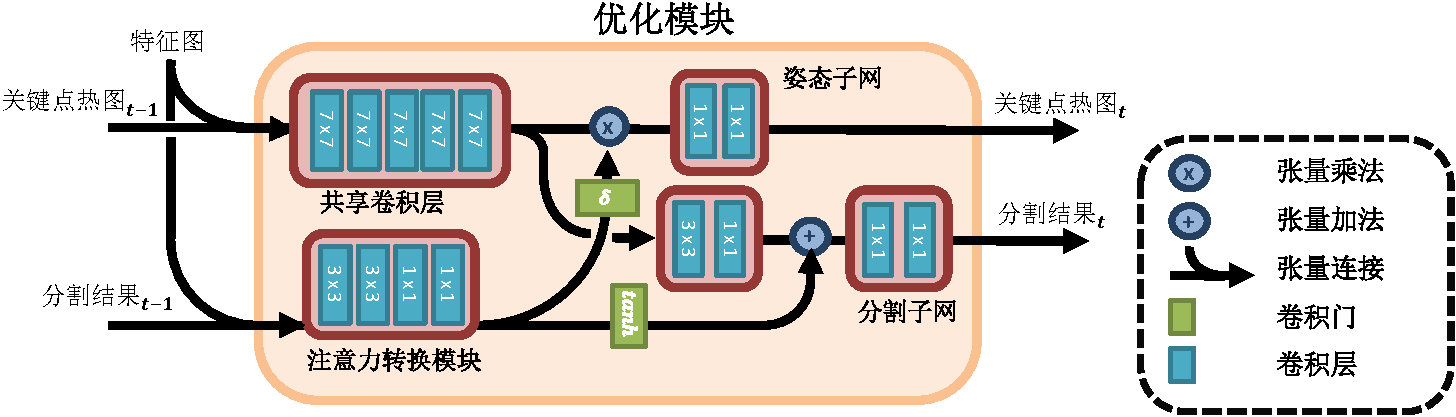
\includegraphics[width=\textwidth]{RefineNet.pdf}
 		\caption{融合优化网络具体设计}
 		\label{fig:RefineNet}
 	\end{figure*}

 	\subsubsection{弱监督与注意力机制}
 	本文使用了弱监督方法约束空间注意力的生成。空间注意力的目标在于获得特定人体的完整区域。实例分割的标注真值未能将被遮挡的人体区域考虑在内,而部分姿态估计真值给出了被遮挡躯干的关键点位置。本文参考了弱监督策略下的学习过程,通过构建间接作用于单通道的空间注意力的损失函数约束,在不完整的标注信息下监督空间注意力的生成。姿态估计信息能够为空间注意力提供结构化的线索,同时实例分割为注意力提供清晰地可见部分的边界监督信息。本文以空间注意力为桥梁设计网络结构,将两任务分支交叉连接,在复合损失函数与单通道结构的共同作用下,间接约束网络生成考虑人体遮挡区域的空间注意力,在空间上选择并强化两任务中对应位置的特征,从而增强多人姿态估计的结果。
 	
 	\subsection{网络训练}
 	本文监督网络的损失函数可以被分为三部分:检测损失函数、关键点分支损失函数与实例分割分支损失函数(具体定义见学位论文)。为了平衡每个分支的收敛速率,本文设计了$\beta$和$\alpha$分别控制目标检测与实例分割的损失函数权重(具体定义见学位论文)。本文提出的优化模块结构涉及到两支子网相互交叉与传递,为了证明网络能够在添加结构的条件下保证两支网络的正常收敛(具体证明见学位论文),给出了损失函数中不同项对于梯度的影响,从而解释了弱监督信息能使用复合损失函数监督注意力的生成。

    \section{实验验证与分析}
	本文在COCO2017数据集上对比了现有方法与本文方法的性能指标,并通过多个对比消融实验证明了本文中提出的核心模块的有效性。

    \subsection{视觉效果与分析}
    \begin{figure}[H]
    	\centering
    	\begin{minipage}{\linewidth}
    		\centering
    		\begin{subfigure}[b]{0.45\linewidth}
    			\centering
    			\begin{minipage}{\linewidth}
    				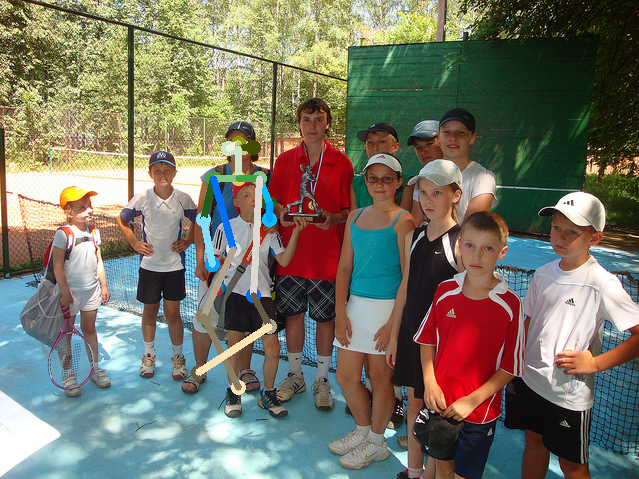
\includegraphics[width=0.48\linewidth]{1000_insid9_stage3_keypoint_baseline.png}
    				\adjustbox{width=0.48\linewidth, trim={.1\width} {.1\height} {.25\width} {.25\height},clip}
    				{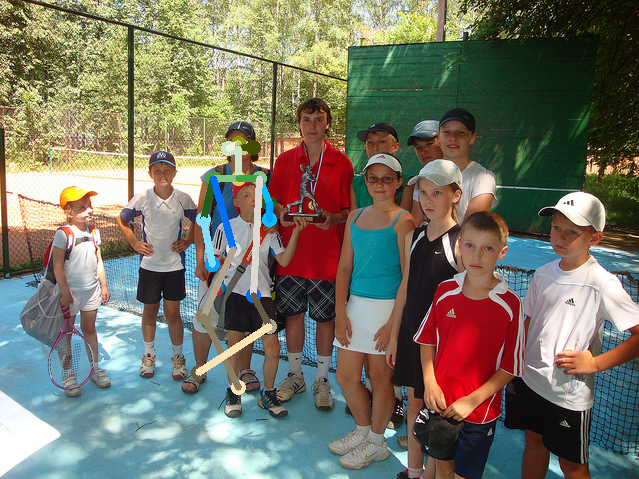
\includegraphics[width=\linewidth]{1000_insid9_stage3_keypoint_baseline.png}}
    			\end{minipage}
    		\end{subfigure}
    		\begin{subfigure}[b]{0.45\linewidth}
    			\centering
    			\begin{minipage}{\linewidth}
    				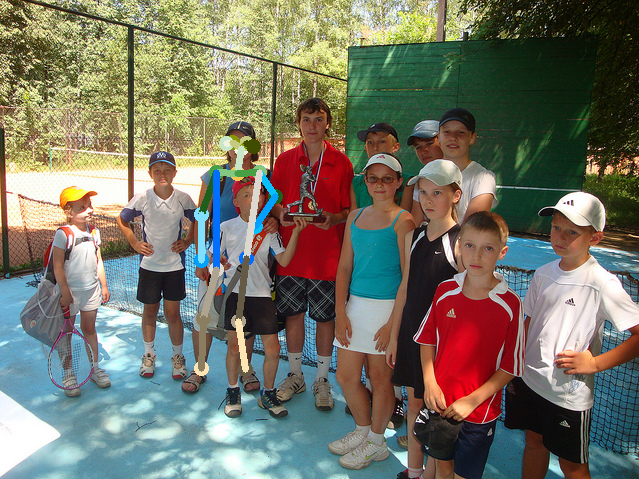
\includegraphics[width=0.48\linewidth]{1000_insid9_stage5_keypoint.png}
    				\adjustbox{width=0.48\linewidth, trim={.1\width} {.1\height} {.25\width} {.25\height},clip}
    				{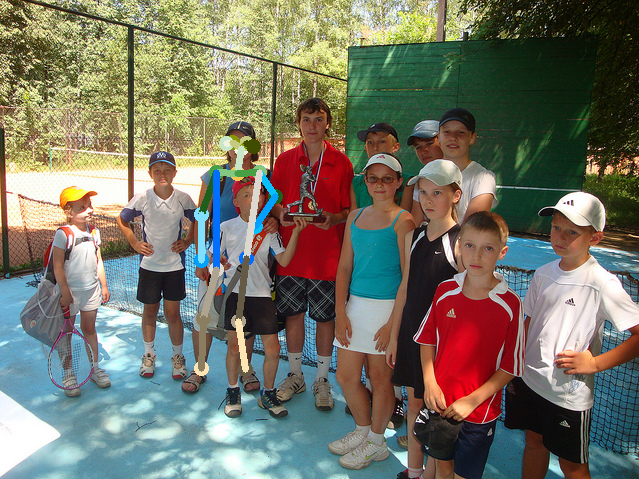
\includegraphics[width=\linewidth]{1000_insid9_stage5_keypoint.png}}
    			\end{minipage}
    		\end{subfigure}
    		
    		\vskip5pt
    		\begin{subfigure}[b]{0.45\linewidth}
    			\centering
    			\begin{minipage}{\linewidth}
    				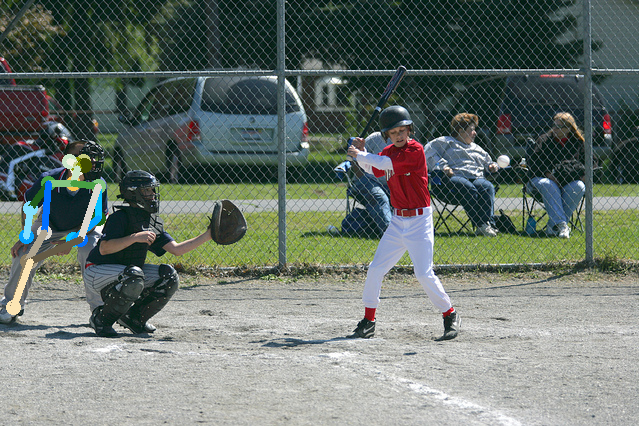
\includegraphics[width=0.48\linewidth]{54593_insid3_stage3_keypoint_baseline.png}
    				\adjustbox{width=0.48\linewidth, trim=0 {.2\height} {.4\width} {.2\height},clip}
    				{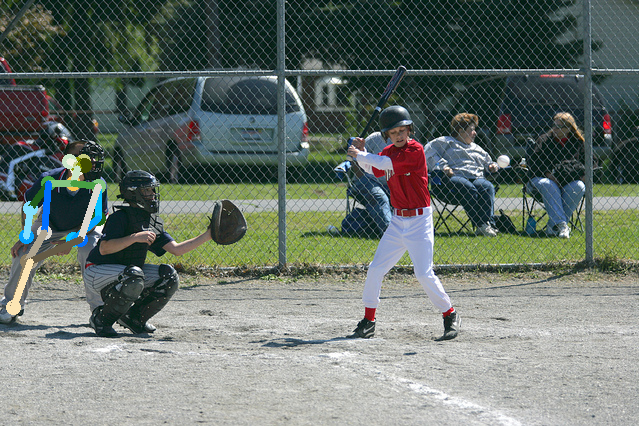
\includegraphics[width=\linewidth]{54593_insid3_stage3_keypoint_baseline.png}}
    			\end{minipage}
    			\caption{基准方法\cite{wei2016convolutional}}
    		\end{subfigure}
    		\begin{subfigure}[b]{0.45\linewidth}
    			\centering
    			\begin{minipage}{\linewidth}
    				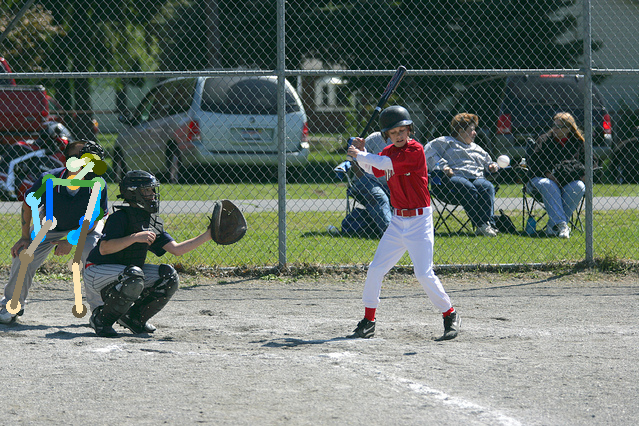
\includegraphics[width=0.48\linewidth]{54593_insid3_stage5_keypoint.png}
    				\adjustbox{width=0.48\linewidth, trim=0 {.2\height} {.4\width} {.2\height},clip}
    				{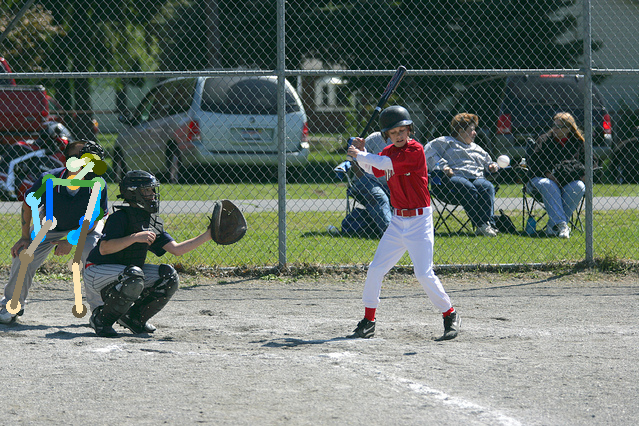
\includegraphics[width=\linewidth]{54593_insid3_stage5_keypoint.png}}
    			\end{minipage}
    			\caption{所提出方法}
    		\end{subfigure}
    	\end{minipage}
    	\caption{本文方法与基准方法关键点任务对比视觉效果图}
    	\label{fig:comparison_keypoint}
    \end{figure}
	如图\ref{fig:comparison_keypoint}所示,本文方法可以比基准方法更好地关注单个实例。通过自生成空间注意力约束,本文方法能够给出更加规整的关键点预测结果,并将结果限制于有限的特定人体区域内。基准方法中给出的多人姿态估计会受到相邻实例的干扰,影响关键点结果的完整性。此外,对于一些完全遮挡下的人体区域,本文方法可以通过注意力生成的关注区域引导姿态分支给出姿态估计。如图\ref{fig:comparison_keypoint}第一行基准方法与本文方法可视化结果对比所示,在注意力的约束下所提出的方法能够排除临近人体躯干的干扰,给出更整齐准确的姿态估计结果。
	
	\begin{figure}[H]
		\centering
		\begin{minipage}{\linewidth}
			\centering
			\begin{subfigure}[b]{0.45\linewidth}
				\begin{minipage}{\linewidth}
					\centering
					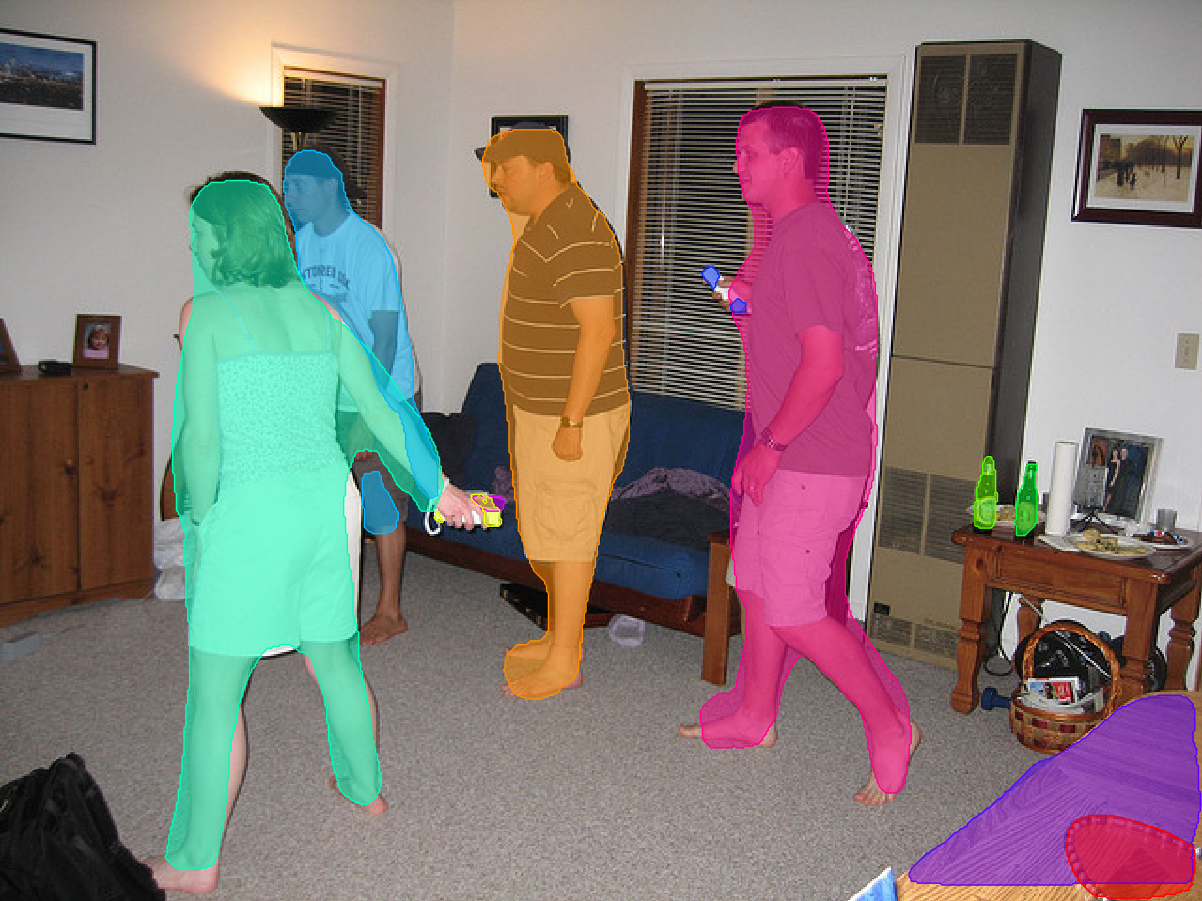
\includegraphics[width=0.48\linewidth]{13729_insid-1_mask_poly_baseline.png}
					\adjustbox{width=0.48\linewidth, trim=0 {.3\height} {0.45\width} {.15\height},clip}%
					{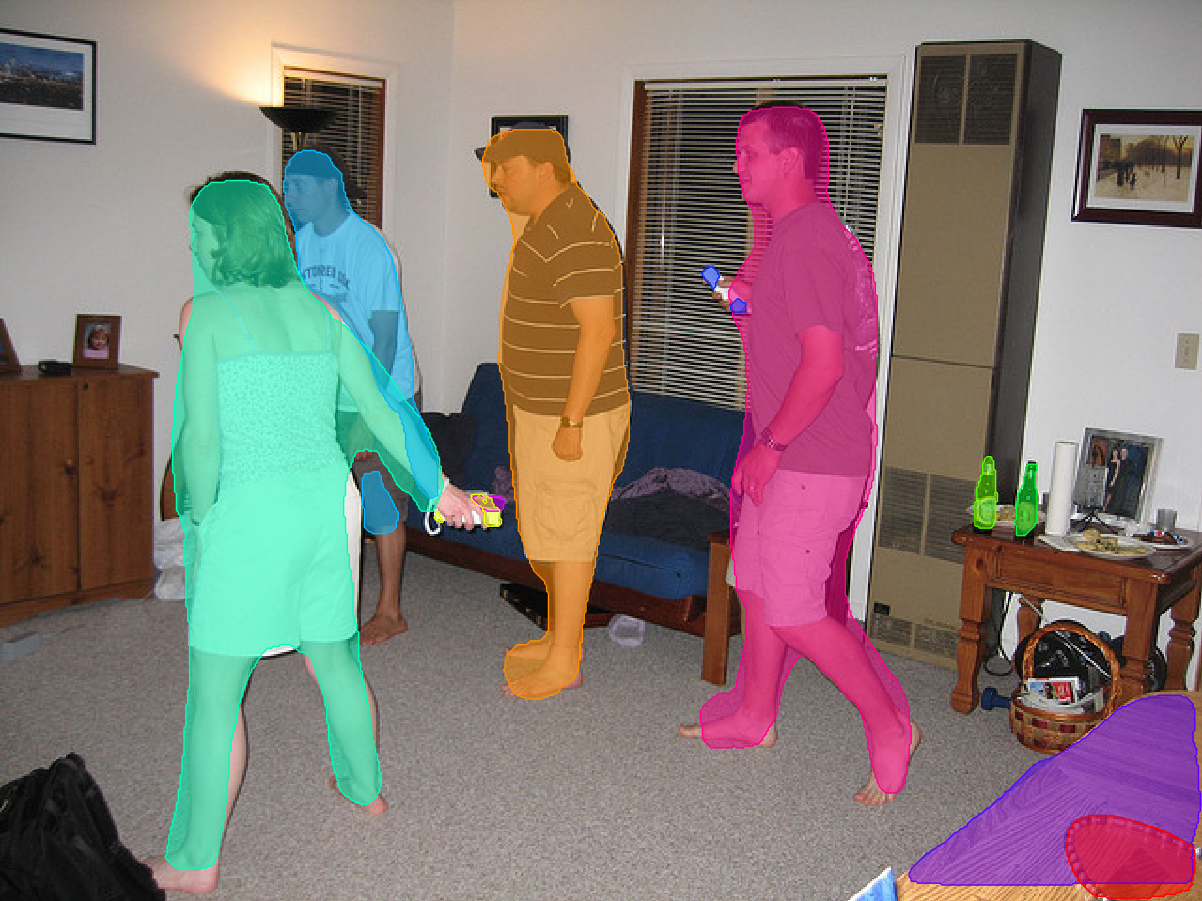
\includegraphics[width=\linewidth]{13729_insid-1_mask_poly_baseline.png}}
				\end{minipage}
			\end{subfigure}
			\begin{subfigure}[b]{0.45\linewidth}
				\begin{minipage}{\linewidth}
					\centering
					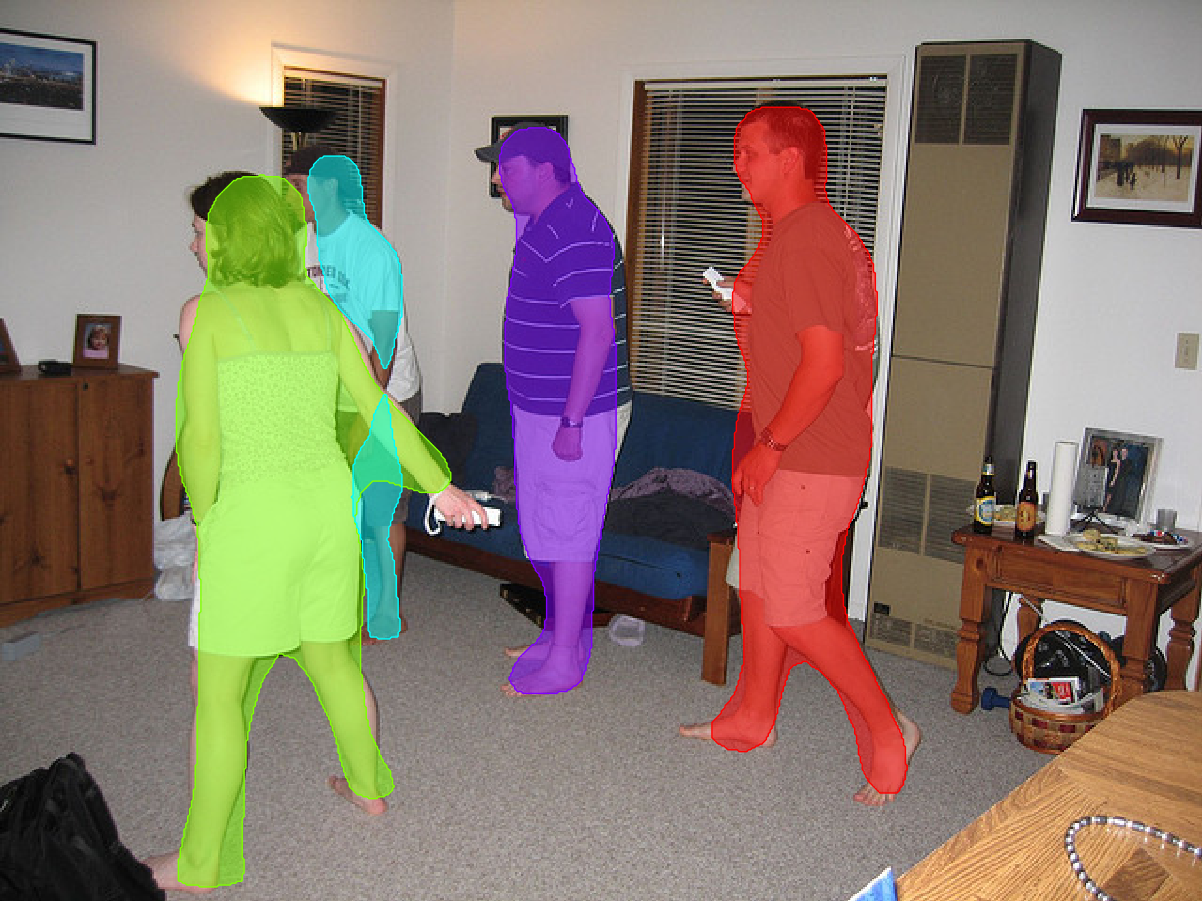
\includegraphics[width=0.48\linewidth]{13729_insid-1_mask_poly.png}
					\adjustbox{width=0.48\linewidth, trim=0 {.3\height} {0.45\width} {.15\height},clip}%
					{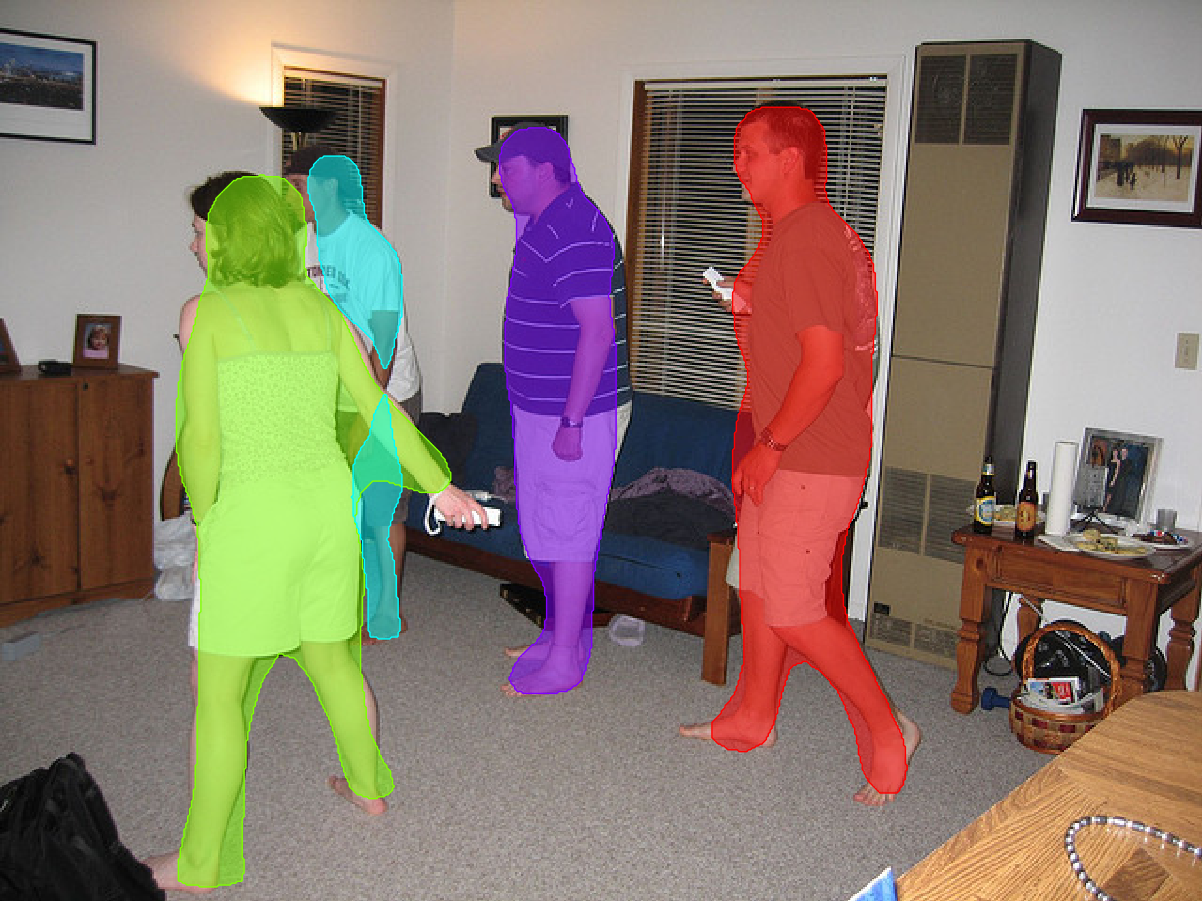
\includegraphics[width=\linewidth]{13729_insid-1_mask_poly.png}}
				\end{minipage}
			\end{subfigure}
			
			\vskip5pt
			\begin{subfigure}[b]{0.45\linewidth}
				\begin{minipage}{\linewidth}
					\centering
					\adjustbox{width=0.48\linewidth, trim={.15\width} {.15\height} {0.15\width} {.15\height},clip}%
					{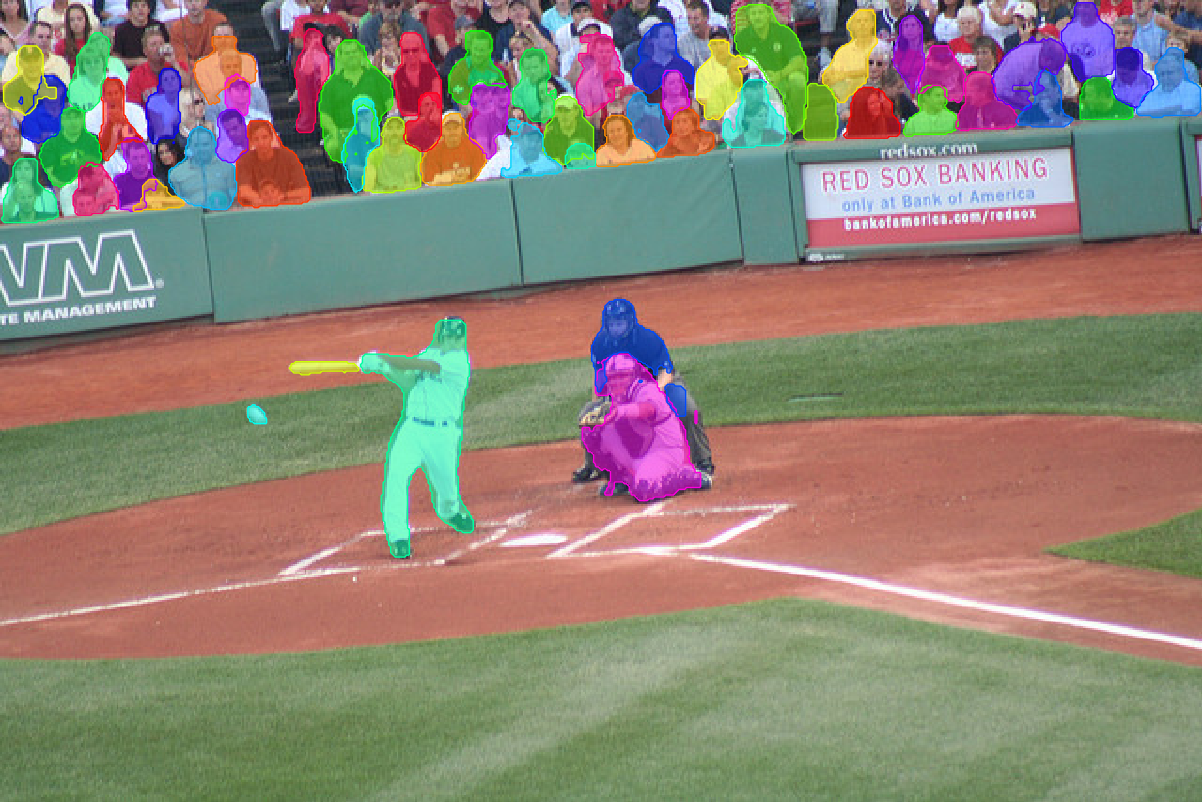
\includegraphics{60507_insid-1_mask_poly_baseline.png}}
					\adjustbox{width=0.48\linewidth, trim={.35\width} {.35\height} {0.35\width} {.35\height},clip}%
					{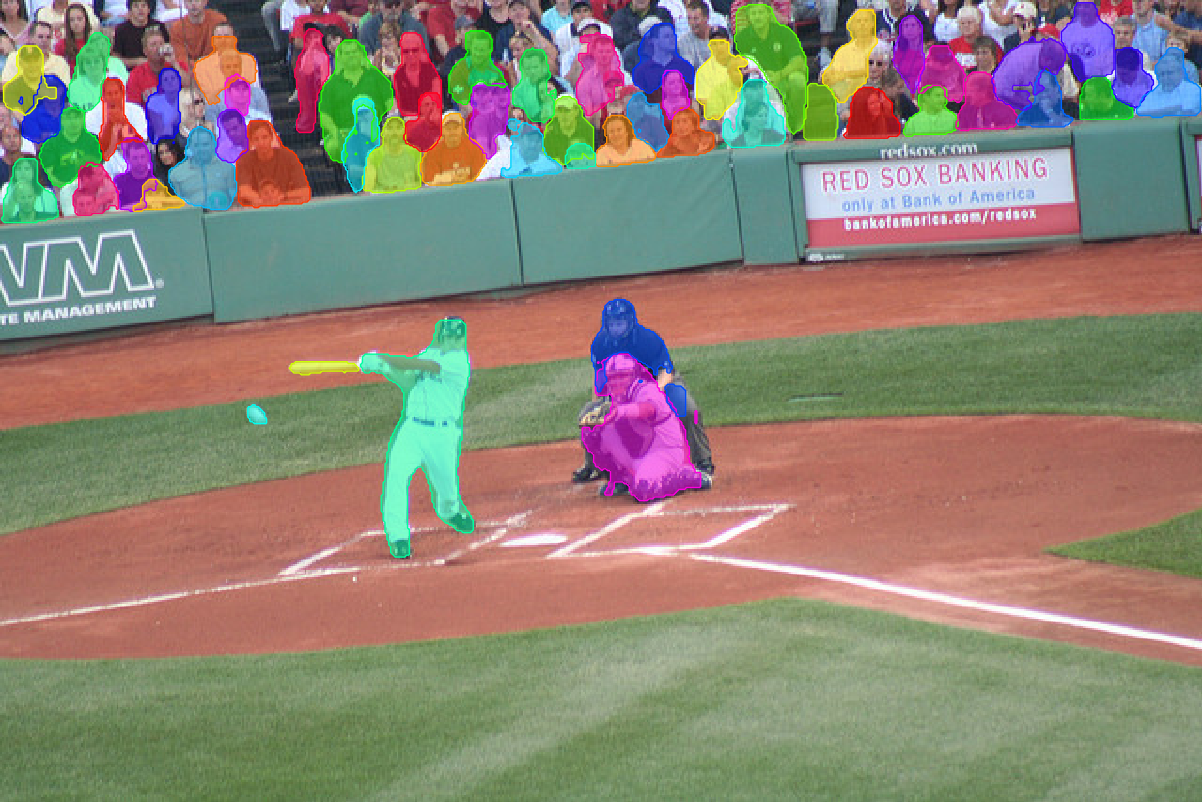
\includegraphics{60507_insid-1_mask_poly_baseline.png}}
				\end{minipage}
				\caption{基准方法\cite{He2017Mask}}
			\end{subfigure}
			\begin{subfigure}[b]{0.45\linewidth}
				\begin{minipage}{\linewidth}
					\centering
					\adjustbox{width=0.48\linewidth, trim={.15\width} {.15\height} {0.15\width} {.15\height},clip}%
					{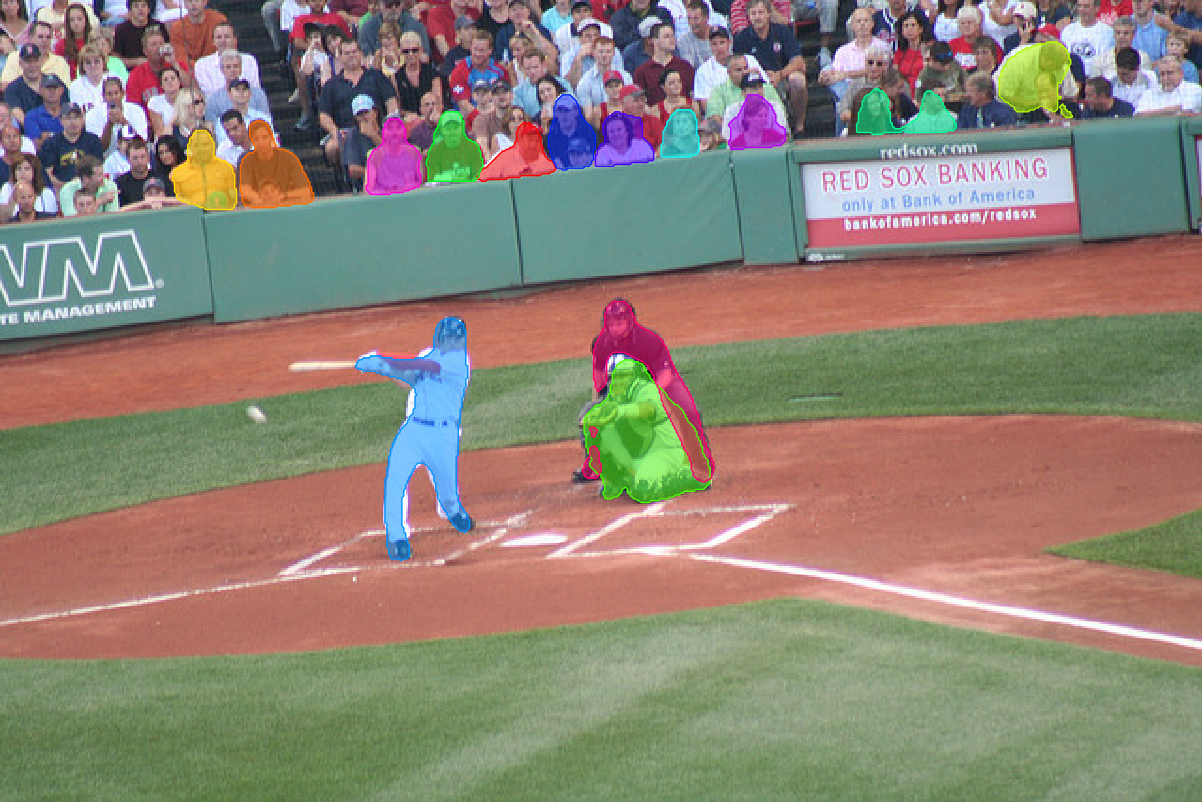
\includegraphics{60507_insid-1_mask_poly.png}}
					\adjustbox{width=0.48\linewidth, trim={.35\width} {.35\height} {0.35\width} {.35\height},clip}%
					{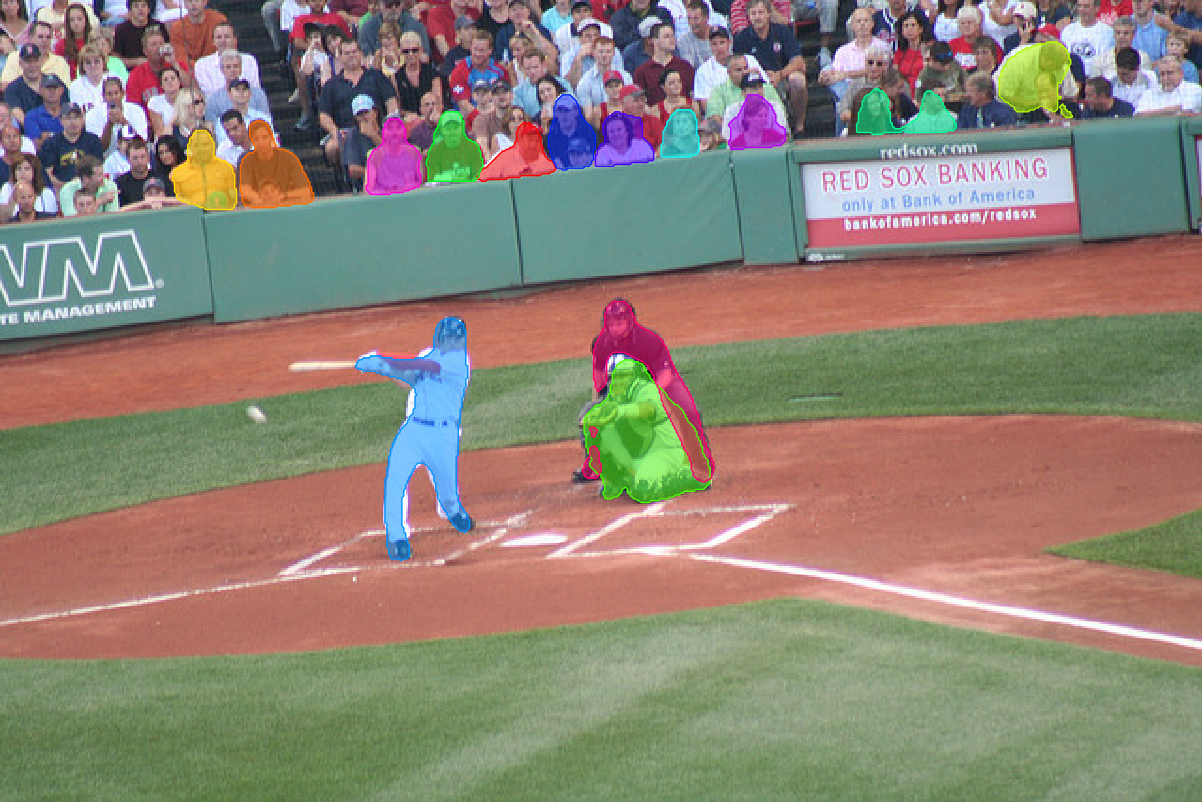
\includegraphics{60507_insid-1_mask_poly.png}}
				\end{minipage}
				\caption{本文方法}
			\end{subfigure}
		\end{minipage}
		\caption{本文方法与基准方法实例分割对比视觉效果图}
		\label{fig:comparison_mask}
	\end{figure}
	如图\ref{fig:comparison_mask}所示,实例分割结果相比于基准方法能够更多地考虑人体全局的特征。在第一行中被手臂遮挡的人体部位在基准方法给出的结果中是上下分离的,并且还出现下半身缺失分割的情况,而在本文方法中,不仅给出了大致结果,同时还连接了一部分断开的身体部分。如图\ref{fig:comparison_mask}中的第二行所示,本文方法给出的实例分割结果对遮挡情况的应对相比基准方法得到了明显的改善。
	

    \subsection{性能对比与分析}
    \begin{table}[H]
    	\centering
    	\caption{COCO测试集的模型性能对比}
    	\label{tab:mAPCOCObenchmark}
    	\begin{minipage}[t]{0.8\linewidth}
    		\begin{tabular}{p{0.25\linewidth}p{0.1\linewidth}<{\centering}p{0.1\linewidth}<{\centering}p{0.1\linewidth}<{\centering}p{0.1\linewidth}<{\centering}p{0.1\linewidth}<{\centering}}
    			\hline
    			方法 & \multicolumn{1}{c}{$mAP$} & \multicolumn{1}{c}{$AP_{OKS=0.5}$} & \multicolumn{1}{c}{$AP_{OKS=0.75}$}
    			& \multicolumn{1}{c}{$AP_M$} & \multicolumn{1}{c}{$AP_L$} \\
    			
    			& \multicolumn{1}{c}{(\%)}& \multicolumn{1}{c}{(\%)}&
    			\multicolumn{1}{c}{(\%)}& \multicolumn{1}{c}{(\%)}& \multicolumn{1}{c}{
    				(\%)}\\
    			\hline
    			堆叠沙漏网络\cite{newell2016stacked} & 46.0 & 74.6 & \textbf{48.4} & 38.8  & \textbf{55.6} \\
    			基准方法\cite{wei2016convolutional} & 41.2 & 71.3 & 45.9 & 34.2 & 47.4 \\
    			所提出方法 & \textbf{46.7} & \textbf{83.4} & 46.6 & \textbf{45.1} & 53.2 \\
    			\hline
    		\end{tabular}
    	\end{minipage}
    \end{table}

	如表\ref{tab:mAPCOCObenchmark}所示,与堆叠沙漏网络相比使用本文提出的优化模块能够显著改善关键点在$AP_{OKS=0.5}$的得分($7.5AP$)。这部分的提升主要是来自空间注意力提供的对人体的精确划分,使得给出的姿态估计更加完整。同时,本文方法在对小目标的姿态检测结果性能$AP_M$上性能较堆叠沙漏网络提高了$4.2AP$。而之后在此基础上额外增加优化模块的本文方法+在原有策略基础上提升$0.8mAP$,在$AP_{OKS=0.5}$与$AP_M$指标上比沙漏网络分别高出$8.8AP$与$6.3AP$。虽然两种优化策略下模型在$AP_{OKS=0.75}$与$AP_L$的指标上超过了复现方法,但不优于沙漏网络给出的评价结果。整体而言,本文方法在$AP$指标上比现有的自顶向下的堆叠沙漏网络高出$0.7mAP$,并能够给出更加完整的姿态估计结果。
	
	\section{结论}
	% 提出结构,有何优势,实验证明
	本文提出一种全新的融合人体实例分割信息的多人姿态检测网络结构。该结构将实例分割信息加入到多阶段的优化网络设计中,同时优化分割结果与姿态估计结果。通过大量定量与定性实验展示网络模型同时给出分割结果和姿态估计结果的性能,并证明本文提出弱监督下空间注意力的有效性。
	
    %% 参考文献
    \bibliography{ref/refs}
\end{outstandingabstract}


% 注意:至少需要引用一篇参考文献,否则下面两行可能引起编译错误。
% 如果不需要参考文献,请将下面两行删除或注释掉。
\bibliographystyle{thuthesis-numeric}      % 顺序编码制
% \bibliographystyle{thuthesis-author-year}  % 著者-出版年制
% \bibliographystyle{thuthesis-bachelor}     % 本科生参考文献的著录格式
\backmatter

\end{document}
